\documentclass{article}

\usepackage[utf8]{inputenc}
\usepackage{enumitem}
\usepackage{graphicx}
\usepackage{tikz, amsmath, amssymb, gensymb}
\usepackage[margin=1in]{geometry}

\title{Project Proposal}
\author{SE464}
\date{\today}

\begin{document}

\begin{titlepage}
\newcommand{\HRule}{\rule{\linewidth}{0.5mm}}

\center

\textsc{\huge University of Waterloo}\\[3cm]
\textsc{\LARGE SE464}\\[1.5cm]
\textsc{\Large Section 001}\\[1.5cm]

\HRule \\[0.75cm]
{ \Huge \bfseries Project Proposal (Revised)}\\[0.5cm]
\HRule \\[2cm]

\Large Group 25 \\  [8cm]

{\Large \today}\\

\vfill
\end{titlepage}

\noindent\textbf{Project Title:} ShuttleQL (Shuttle Queueing Logistics) \\
\textbf{Team Members:}
\begin{itemize}
  \item Cheng Dong (c9dong)
  \item Zhaotian Fang (z23fang)
  \item Clement Hoang (c8hoang)
  \item Di Sen Lu (dslu)
\end{itemize}

\section{Introduction}
\subsection{Motivation}
Around the world, there are 100s of recreational badminton clubs which host
regular sessions at set locations for members to drop in and play at.
Traditionally, the operation of a badminton club was done manually through the
combined efforts of the clubs executive staff. There are several burdenous
and repetitive tasks that the staff members need to do on a regular basis in
order to keep the club running smoothly. For example,
\begin{itemize}
  \item Registering new club members
  \item Checking in/out members during a club session
  \item Scheduling members into courts for each rotation
\end{itemize}
These tasks negatively impact the productivity of the staff and are prone
to human error.
In addition, there is no effective means for the club execs to communicate
with the members in real-time.
Finally, there is no easy way for a member to get feedback on their own performance
unless they hire a coach or ask for critique from a staff member.

\subsection{Idea}
ShuttleQL is an all-in-one badminton club management platform which not only
automates repetitive administrative tasks but also acts as a communication hub
between the club executives and its members. It also offers insights and
analytics into performance of the players in the club. \\

The platform will be entirely web-based. It will consist of two components:
a club member mobile web based dashboard and an admin desktop web based dashboard.
The platform from the club member's perspective will be a mobile web based app
since they are more likely to have access to a phone than a laptop when they
come to session. The admin dashboard will be desktop web based since it requires
heavy user interaction which will be easier on a laptop rather than on a phone.

\subsection{Originality}
Although existing software solutions exist for a similar purpose, they are often
incomplete relative to ShuttleQL and don't leverage many of todays technologies.
ShuttleQL aims to fix most if not all of the pain points associated with
managing a badminton club. It also applies new concepts such as data analytics and
machine learning into processes such as matchmaking and coaching, which has not
yet been done in existing solutions.

\newpage

\section{Project Properties}
\subsection{Functional}
\begin{enumerate}
  \item Registering new club members
  \item Allowing users to check-in/check-out of a club session
  \item Match making algorithm that allocates players to open badminton courts
  \item Display current players that should be on each court
  \item Allow executives to override the match making algorithm
  \item (Bonus): Send notifications to users once they are able to play
  \item (Bonus): Allow executives to broadcast announcements to users
  \item (Bonus): Show the match history of each member
  \item (Bonus): Track match-making-rating of club members in ladder matches
\end{enumerate}

\subsection{User Scenarios}
There are two different types of users in our system. The first type of user is
a badminton club executive. They have access to a variety of different admin-level
actions such as player management, court management, and communication.
For example, they can override the match making done by system. This will be useful
in the scenario that a member is scheduled to play on a court but they have to leave
early, so the executive can simply replace the member that's leaving with a new
member that isn't playing. \\

The second type of user is the normal badminton club members. They would interact
with our system by viewing on their phones the current players playing on each court.
This reduces crowding between rotations if this information was displayed in on
centralized location in real life. In addition, they get notifications when
it's their turn to play. Using notifications eliminates the need for the member
to constantly check whether they are playing or not.

\subsection{Non-functional}
The two mandatory non-functional properties that our system needs to support are dependability and portability.
The other non-functional properties are bonuses.

\subsubsection{Dependability}
Dependability describes the reliability of the system.
It also describes how accurate the software features meets the specifications.
The system should behave exactly as the specifications describe without encountering any software bugs.
This property is important because our system needs to be reliable for every badminton club session.
It is crucial that every user has correct matches in order to have good user experience. \\
\textbf{Requirement:} The system must have an uptime of 95\% or better for every 24 hours.

\subsubsection{Portability}
Portability refers to the ability of a system to execute on multiple platforms while
retaining its functional and non-functional properties. \\
\textbf{Requirement:} The user-facing interface should, at a minimum, satisfy functional properties 1-4 on
a number of different platforms and browsers. For mobile phones, it should support Chrome on Android and Safari on iOS.
On laptops/desktops, it should support both Chrome and Safari.

\subsubsection{(Bonus) Efficiency}
Efficiency describes the system's performance requirements.
The match making algorithm should run as fast as fast as possible to minimize
the time it takes to generate a new set of matches. \\
\textbf{Requirement:} The match-making algorithm should take less than 5 seconds to complete given a pool
of 100 badminton players.

\subsubsection{(Bonus) Evolvability}
Adaptability describes how well the system adapts to new requirements to the software.
Every time that a new requirement is introduced into one component of the system,
other components of the system should still function correctly without needing intervention.
This property is important to our system since the requirements may change based on the badminton club over time. \\
\textbf{Requirement:} The system should be adaptable to clubs with different number of courts and different game types
for each court.

\newpage

\section{Mockups}
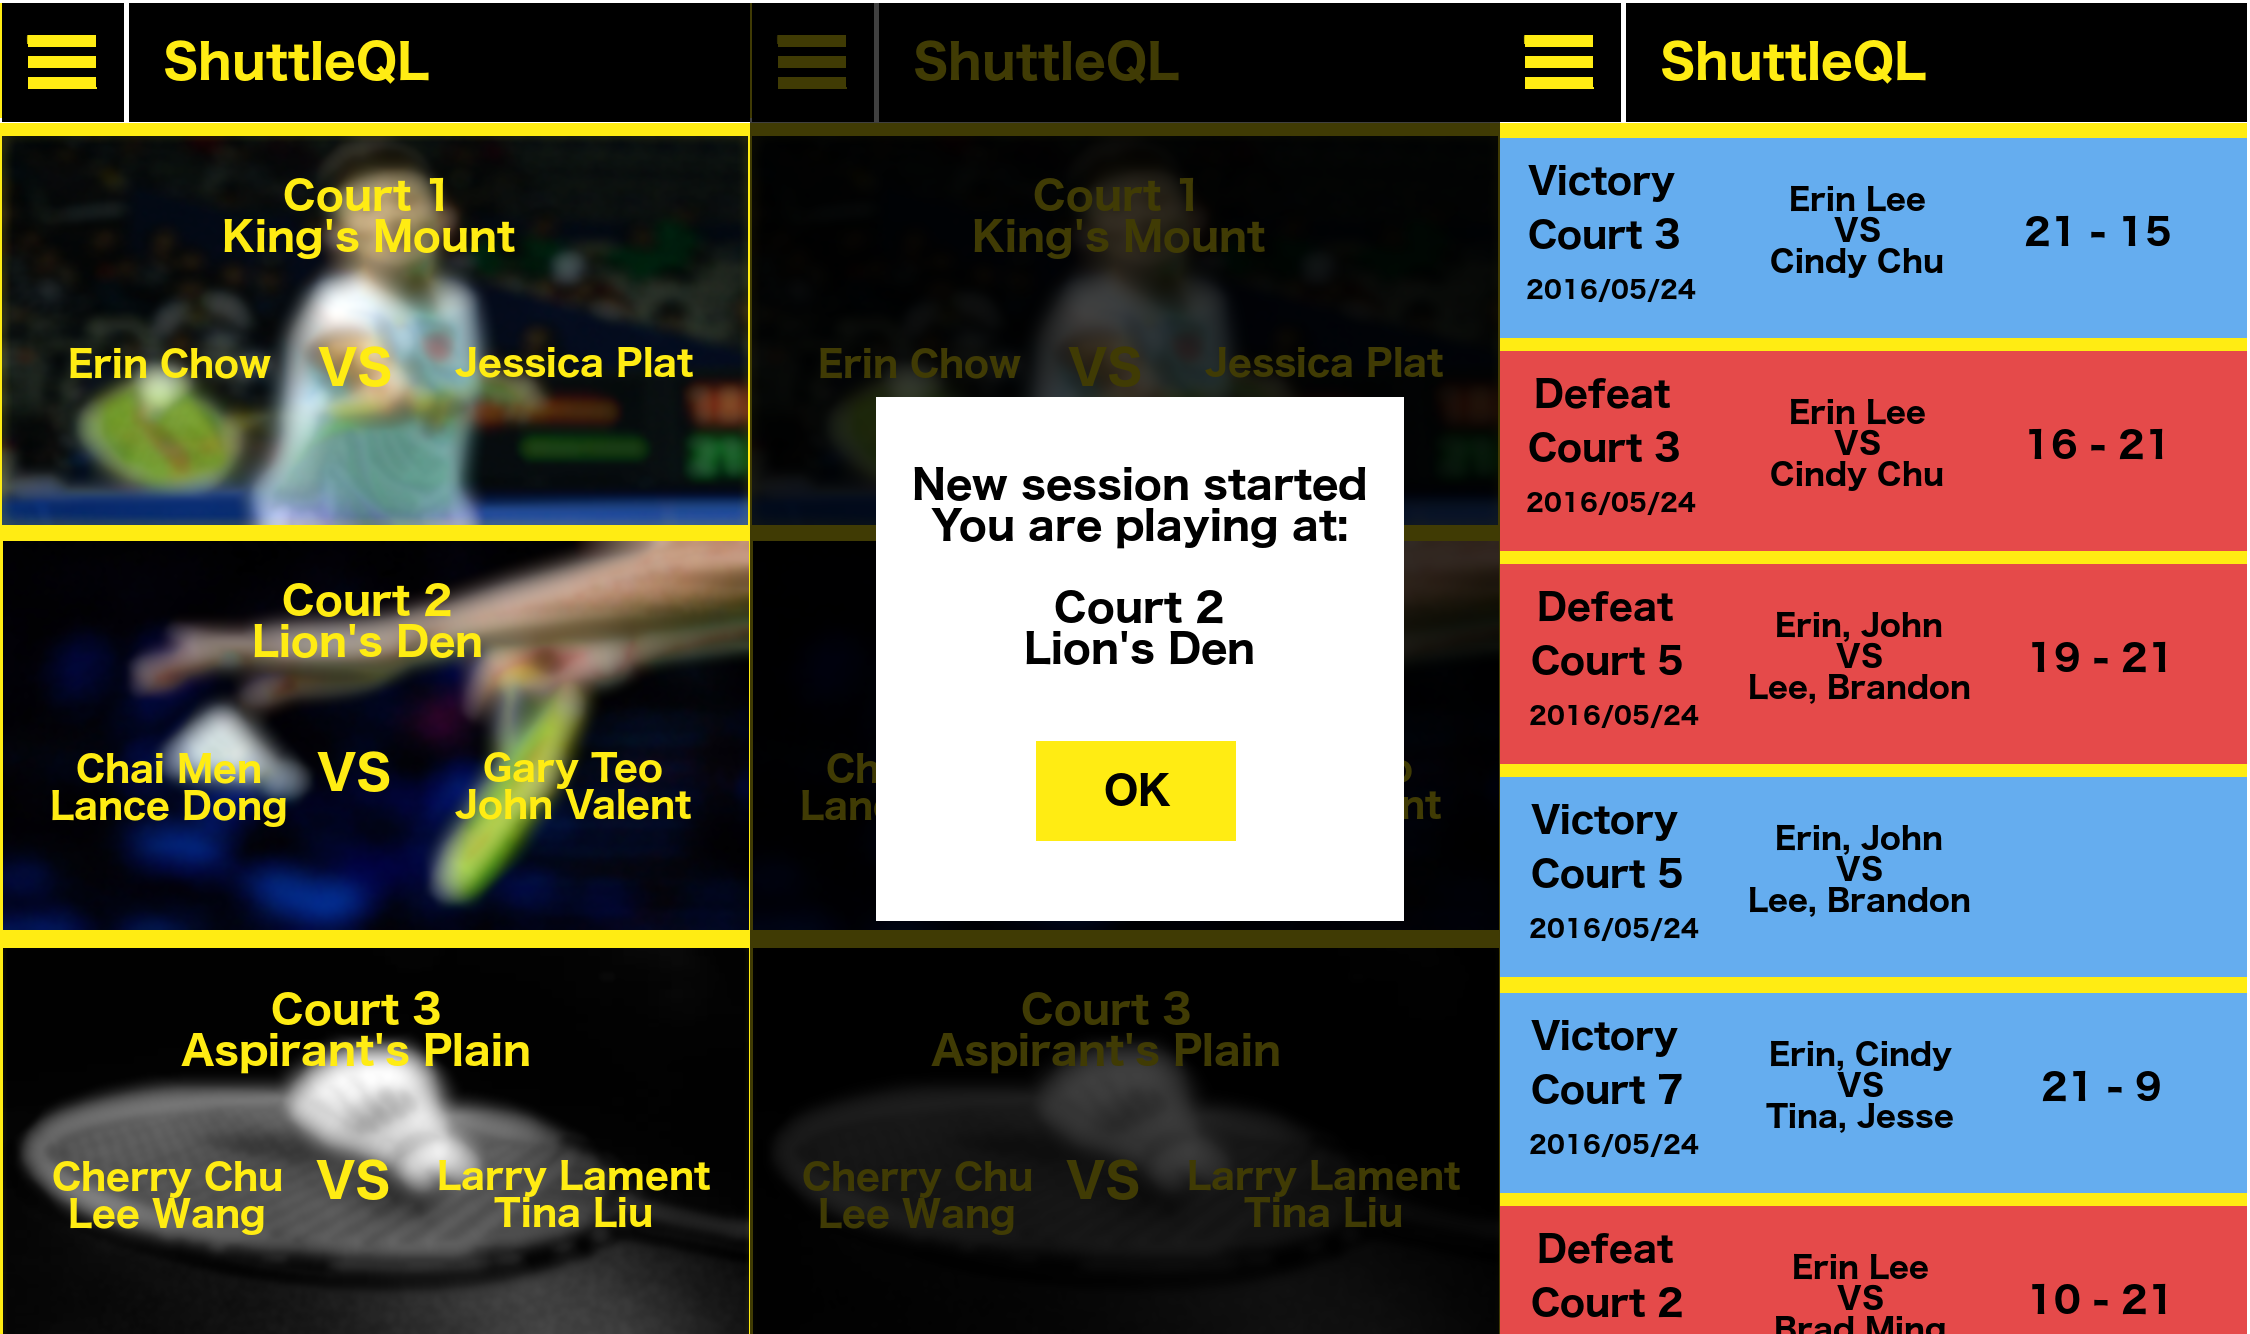
\includegraphics[width=15cm]{combined}

\end{document}
